\documentclass{article}

\usepackage{amsmath}
\usepackage[english]{babel}
\usepackage{graphicx}
\usepackage{natbib}
\usepackage[utf8]{inputenc}
\usepackage[font=small,labelfont=bf]{caption}
\usepackage{booktabs}
\newcommand{\tabitem}{~~\llap{\textbullet}~~}

\setlength{\parindent}{2em}
\setlength{\parskip}{1em}

\title{Homology benchmarking: it's such a BLAST! \\ \large Just don't GO there.}
\author{
	Thomas Braam [2051176]
    \and
    Harmen Boers [2581619]
    \and
    Annalisa Carli [1894536]
    \and
	Olivier Martin [2576272]
    \and 
    \small All authors of group D contributed equally to this project.}
    
\date{\today}

\begin{document}

\maketitle

\begin{abstract}

Many protein sequences have unknown structure, function and evolutionary relations. Homologs can tell us something about the structure or function of a protein because they share a common ancestor. BLAST and PSI-BLAST are established methods used to find homologs using sequence data. However, their performance has not been fully investigated. In this study, we aimed to benchmark the performance of BLAST and PSI-BLAST to Gene Ontology as a gold standard. We used coverage and error to produce receiver operator characteristics plots, resulting in an area under the curve of 0.676 for BLAST and 0.679 for PSI-BLAST. Our results indicate that BLAST and PSI-BLAST have relatively low and similar accuracy for homology prediction. Therefore we can conclude that BLAST and PSI-BLAST perform far from optimal in searching for homologs. However taking into account 87 pairs of false positives with low BLAST and PSI-BLAST E-values, GO is probably not yet annotated enough to serve as a homology benchmarking standard. So might our gold standard actually be silver?

\end{abstract}

\newpage
\tableofcontents

\newpage
\section{Introduction} 

Protein diversity is the result of evolution. The level of diversity can be ascribed to the course of evolution. Proteins with shared ancestry are called homologs. There are two types of homologs: orthologs and paralogs. Orthologs are genes originating from a single ancestral gene in the last common ancestor of the compared genomes. Paralogs are genes related via duplication \citep{koonin_orthologs_2005} (Figure \ref{fig:homology}) [Q2.1]. Homology searches of protein or nucleotide sequences can give insight into protein structure, function, evolutionary relations, and identification of gene families. There are different ways to search for homology in bioinformatics; wherein algorithms find regions of similarity between sequences, structure or function.

\begin{figure}[!ht]
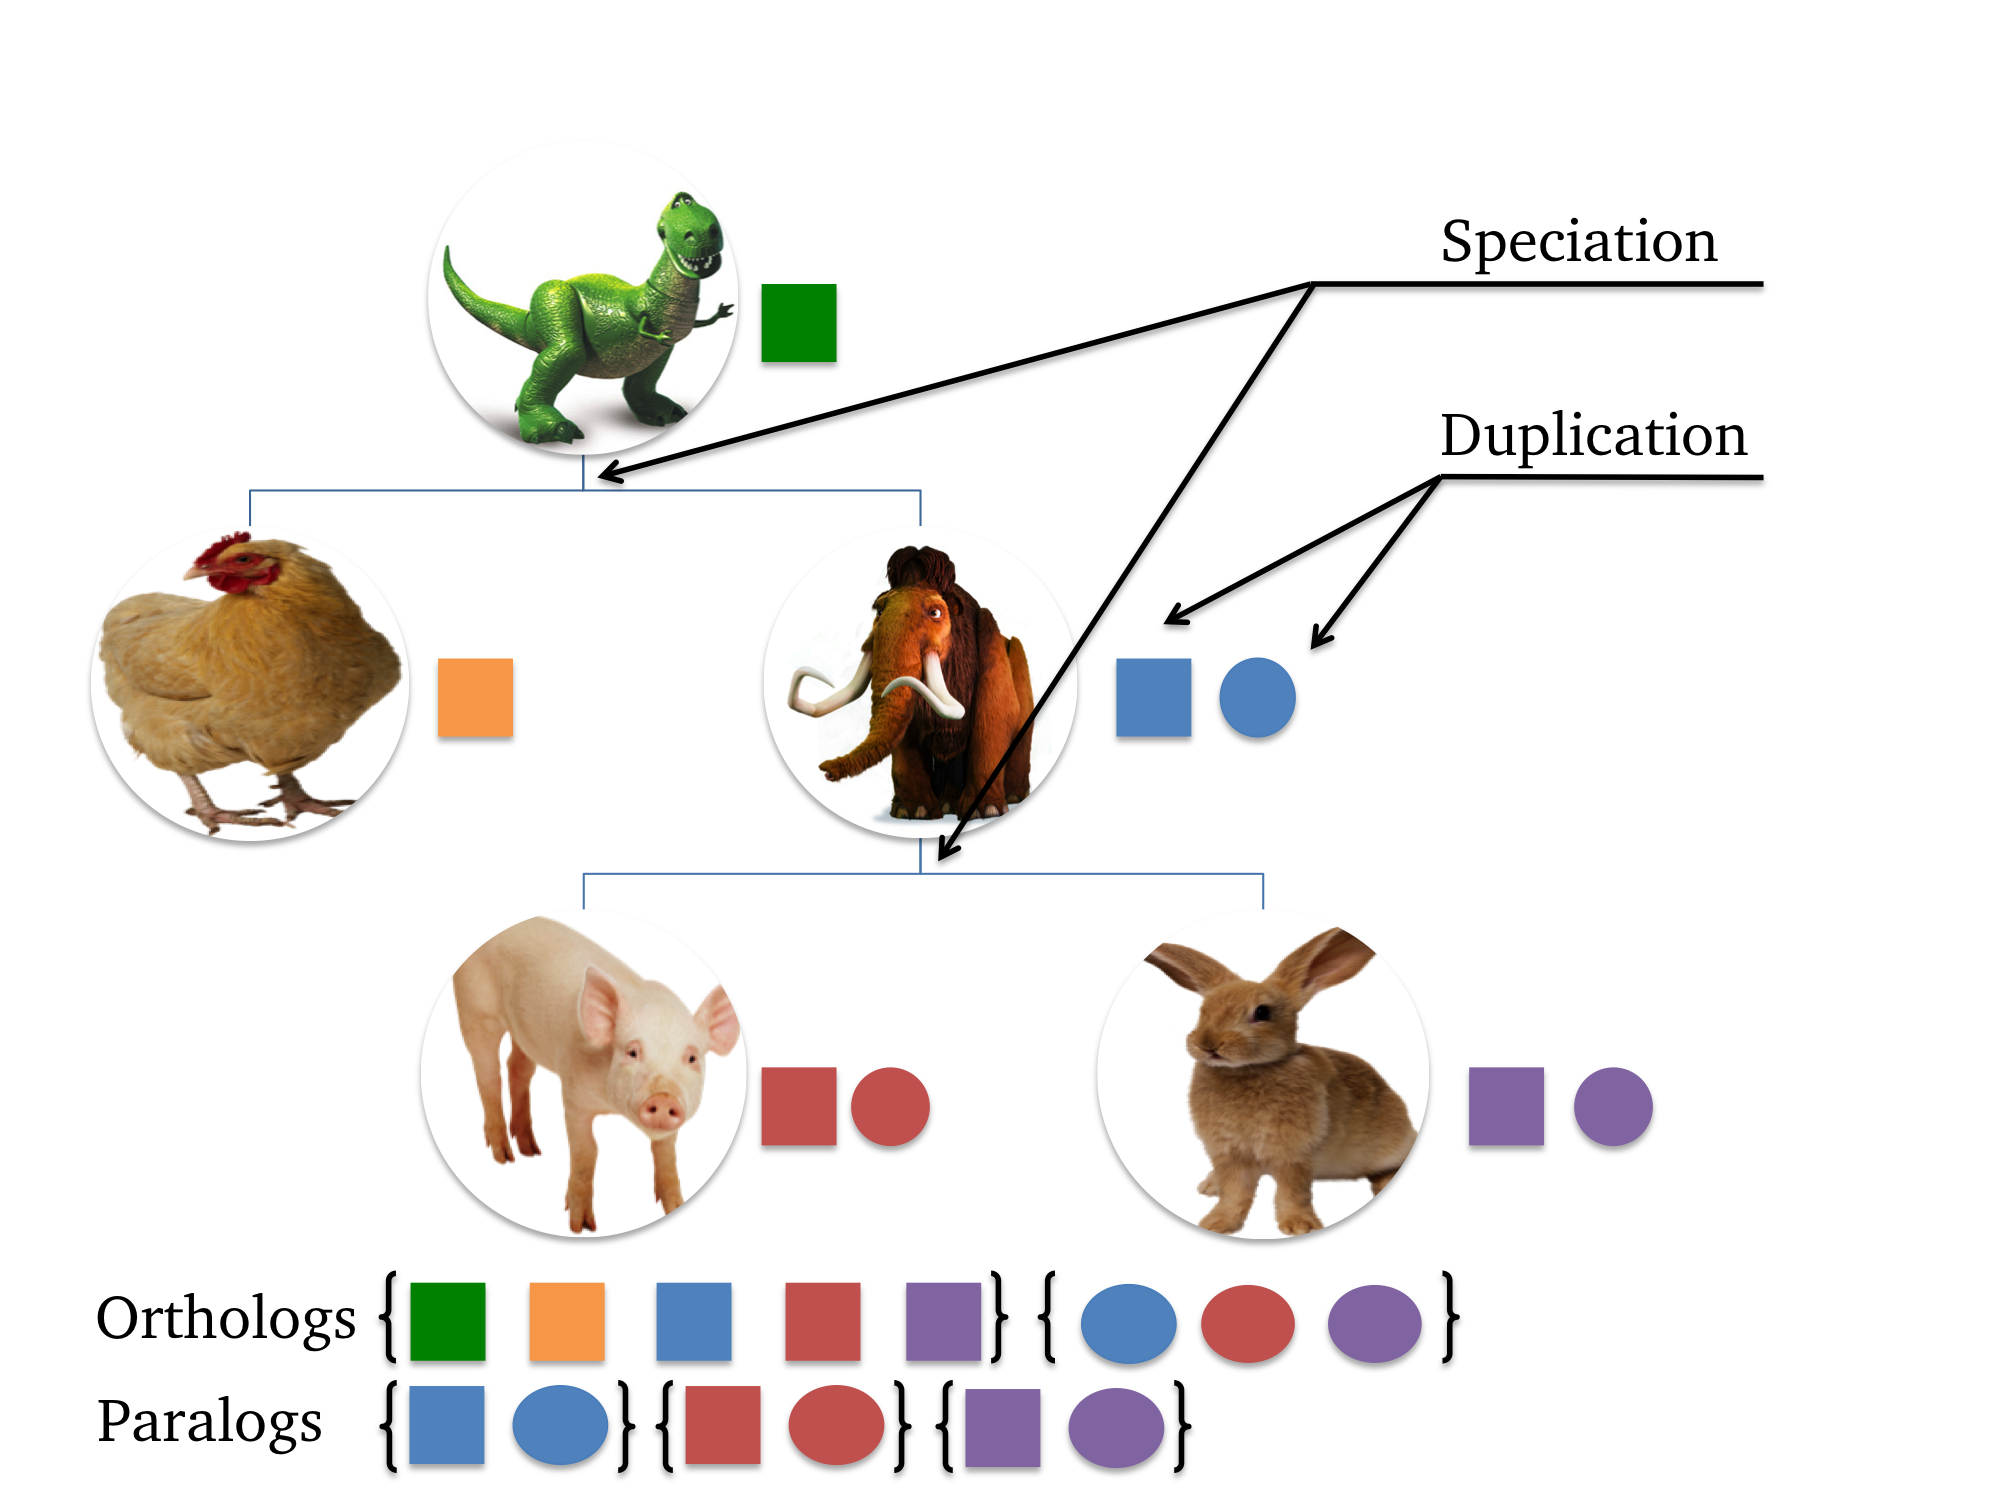
\includegraphics[width=\linewidth]{homology}
\caption{\textbf{Hypothetical evolution tree.} A single gene (square) evolves through a speciation event (change of color) or a duplication event (addition of circle). Wherein the same gene between species (all squares or all circles) are orthologs. Paralogs are the genes related due to a duplication event within one species.}
\label{fig:homology}
\end{figure}

\newpage
A common tool to find homology is the Basic Local Alignment Search Tool (BLAST). This program compares the query nucleotide (DNA) or amino-acid (protein) sequences to a sequence database and reports those alignments that score above a given E-value threshold. Position Specific Iterative BLAST (PSI-BLAST) uses an iterative process where the first iteration is identical to BLAST and returns a list of hit sequences. Hit sequences above a certain E-value threshold are used to compute a Position-Specific Scoring Matrix (PSSM). This PSSM is then used to query the database in the following iteration. New hits are then added to the PSSM. This continues until desired or until convergence (\textit{i.e.} the state where no new sequences are detected above the defined threshold).\citep{bhagwat_psi-blast_2007}, \citep{bergman_comparative_2007}. BLAST is therefore commonly used to find close homologs and PSI-BLAST to search for more distant homologs [Q2.1 + Q2.2].

Gene Ontology (GO) is a database that aims to annotate consistent descriptions of gene products in a species-independent manner \citep{ashburner_gene_2000}. Three ontologies describe gene products in terms of their associated biological processes, cellular components and molecular functions \citep{smith_ontology_2003} [Q3a1]. A protein can be assigned to several GO terms. This is useful to obtain more information about the protein by describing different aspects of the protein function, location or process it is involved in. The rationale behind GO is that it includes the relations of the GO ontologies as well as the annotations of genes and gene products to their GO terms, therefore making GO a powerful relational database \citep{ashburner_gene_2000} [Q3a2+3]. In addition to GO, other databases annotate different protein properties. Pfam is a database where protein sequences are scanned for multiple sequence alignments using hidden Markov models. The proteins are grouped in families known as clans. As the determination of the clans is an automated process, a lot of proteins have been indexed in the Pfam database (40,000,000) \citep{finn_pfam_2014}. SCOP is a database where proteins are grouped in families and superfamilies by their secondary structure, structural folds, evolutionary relations and sequence similarity. The SCOP database is however smaller in size (40,000) \citep{conte_scop_2000}.

During evolution, protein structure is more relevant than its primary sequence for protein function. This results in more conserved protein structures rather than sequences. This implies that different protein sequences can have the same protein structure and, therefore, similar function. These conserved structures, without similar sequence, are not found by BLAST. However, PSI-BLAST has been demonstrated to be useful in detecting such relationships via sequence searches, which previously only could be detected through direct comparison of the structures \citep{bhagwat_psi-blast_2007}. The aim of our study is to benchmark BLAST and PSI-BLAST as a homology search tool by comparing it to GO as a gold standard.

\newpage
\section{Materials \& Methods}
\subsection{Setting up a local sequence database}

A list of 209 UniProtIDs was used to download corresponding protein sequences in fasta format from the UniProt database \citep{consortium_uniprot:_2015}. A fasta file containing all sequences was used to generate a local sequence database for BLAST and PSI-BLAST using the formatdb command. The three generated files had the following extensions: .phr .pin .psq. The size of the database had an influence on the amount of computation needed (time and memory) and on the significance of alignments (more sequences implies a greater probability of getting a match) [Q1]. A simplified summary of the methods is shown in figure \ref{fig:flow_chart}.

\begin{figure}[!ht]
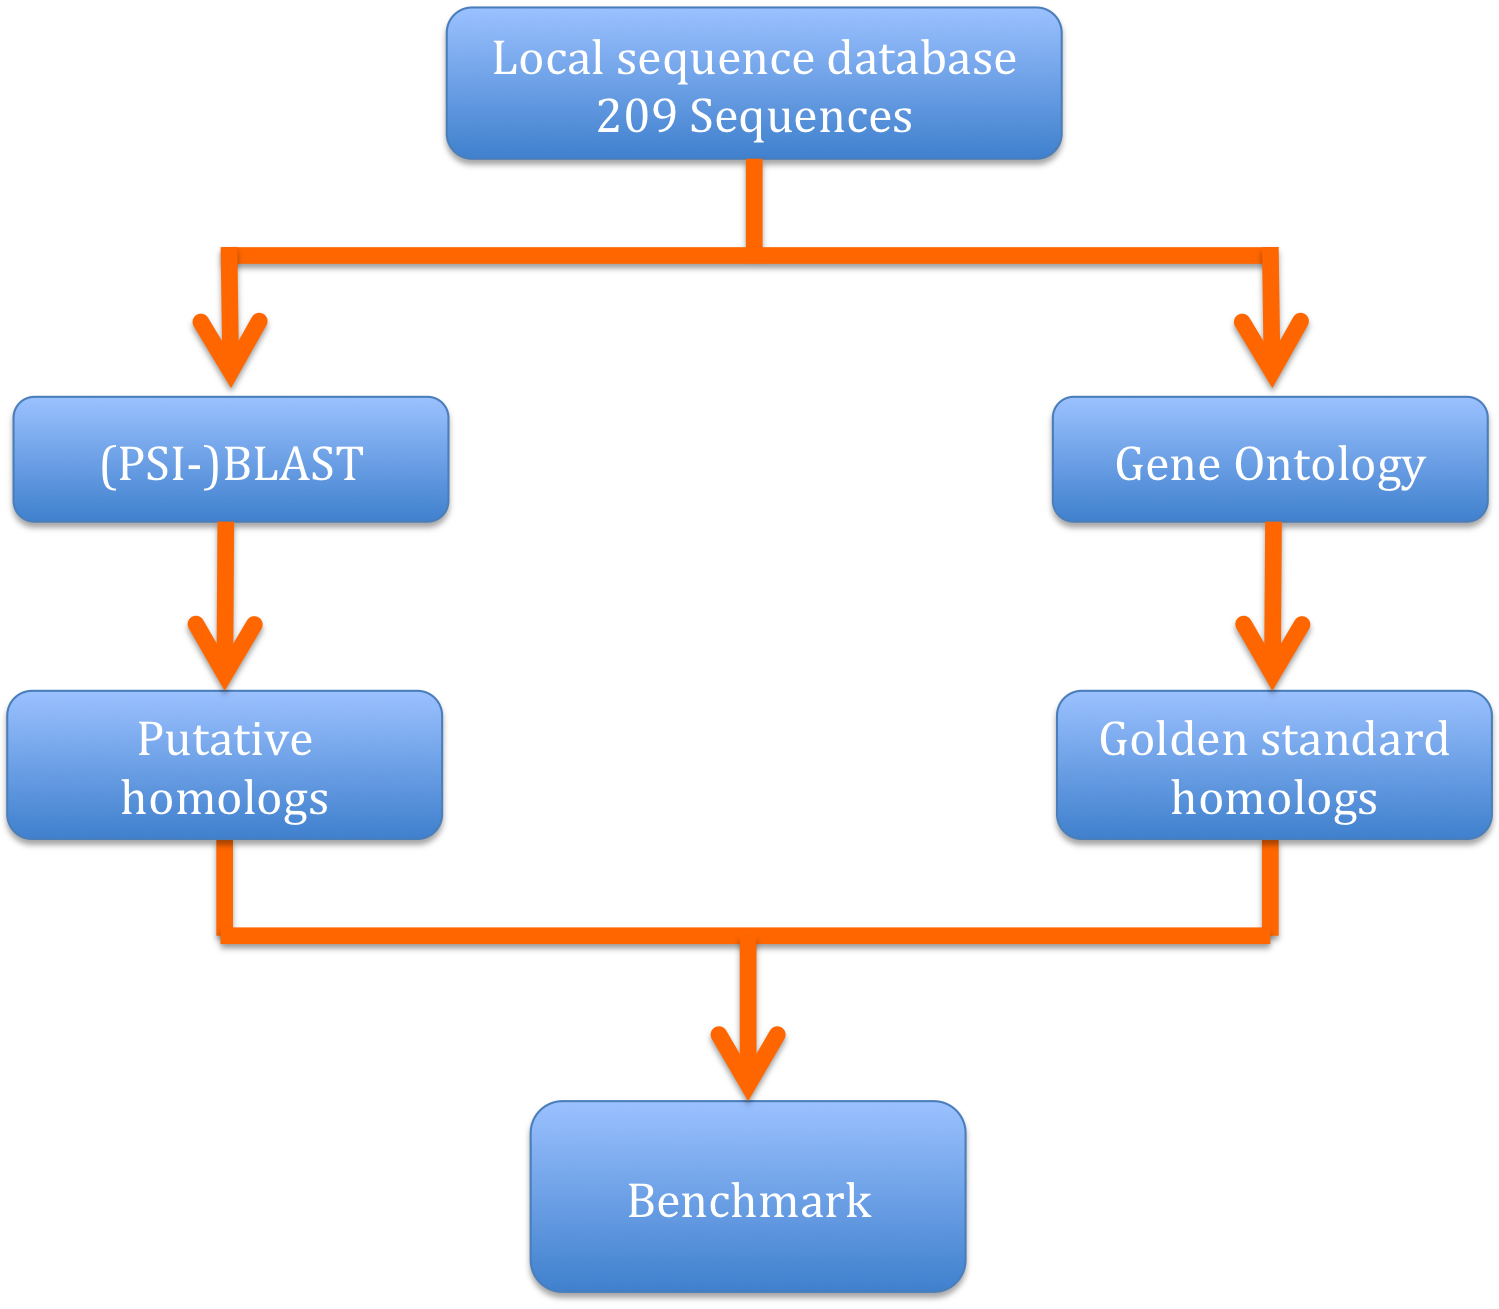
\includegraphics[width=\linewidth]{flow_chart}
\caption{\textbf{Flow chart: simplified summary of materials and methods.} For each protein pair of the local sequence database, putative homologs were found using BLAST and PSI-BLAST. Gold standard homology was defined using similarity between Gene Ontology molecular function. BLAST and PSI-BLAST results were benchmarked according to this gold standard.}
\label{fig:flow_chart}
\end{figure}

\subsection{Finding putative homologs}

The sequence similarity of each protein pair was evaluated with BLAST and PSI-BLAST. The threshold E-value for which pairwise sequence alignments are reported in the output (specified with the -e argument) was set to $10^{4}$. If an alignment was not reported (\textit{i.e.} E-value $> 10^{4}$), the corresponding E-value was set to $10^{6}$. The threshold E-value for inclusion in the PSSM in the next iteration (specified with the -h argument in the case of PSI-BLAST) was set to 0.005 [Q2.5]. The number of iterations of PSI-BLAST (specified with the argument -j) was set to three. The specified number of iterations does not necessarily match the actual number of iterations. For example, if, after an iteration, no sequences were added or removed from the PSSM, then the algorithm would not run another iteration. The returned results would be identical because the algorithm has converged [Q2.4].

For each protein pair, a raw score $S$ of similarity was computed using the BLOSUM62 substitution matrix \citep{henikoff_amino_1992}. The raw score was normalized into the bit score $S'$, allowing comparison of scores obtained using different databases and scoring systems. The bit-score was computed according to formula \eqref{eq:bitscore} where $K$ and $\lambda$ are scale parameters \citep{altschul_basic_1990}. A high bit-score indicates high similarity between sequences [Q2.3].

\begin{equation}
S' = \frac{\lambda S - \ln K}{\ln 2}
\label{eq:bitscore}
\end{equation}

To evaluate the statistical validity of the alignment, an E-value was computed. This E-value corresponded to the number of alignments with a raw score of at least $S$. It was computed using formula \eqref{eq:evalueraw} where $K$ and $\lambda$ are scale parameters, $m$ is database length and $n$ is the query sequence length \citep{altschul_basic_1990}.

\begin{subequations}
\begin{align}
E &= K m n e^{\lambda S} \label{eq:evalueraw} \\
&= m n 2^{-S'} \label{eq:evaluebit}
\end{align}
\end{subequations}

\subsection{Gene Ontology as a gold standard}
\label{sec:gold}

Since structure, and thus function, is more conserved than sequence, functional similarity was used as a gold standard to assess whether two proteins were truly homologous. Gene Ontology annotations for each protein were retrieved automatically. Functional similarity $s$ between each protein pair $p_i, p_j$ was computed with formula \eqref{eq:go} where $g(p_i)$ is the set of GO annotations of protein $p_i$. The minimal score of 0 indicates no common shared functionality while the maximal score of 1 indicates complete functional identity (\textit{e.g.} comparing a protein to itself). 

\begin{equation}
s(p_i, p_j) = \frac{g(p_i) \cap g(p_j)}{g(p_i) \cup g(p_j)}
\label{eq:go}
\end{equation}

In order to determine a threshold to assert homology between a protein pair, the distribution of Gene Ontology scores were estimated by randomly selecting 1000 human proteins from UniProt (Figure \ref{fig:go_random_density}). Protein pairs with a score below the 95\% quantile random distribution quantile ($s = 0.14$) were considered as different. Proteins with a score above the 99\% quantile ($s = 0.27$) were considered as similar. Protein pairs with intermediate scores (\textit{i.e.} between $0.14$ and $0.27$), or absence of GO functional annotations for any of the two proteins were considered as having an ambiguous relation. These ambiguous pairs were ignored for further analysis [Q3a.4].

\begin{figure}[!hb]
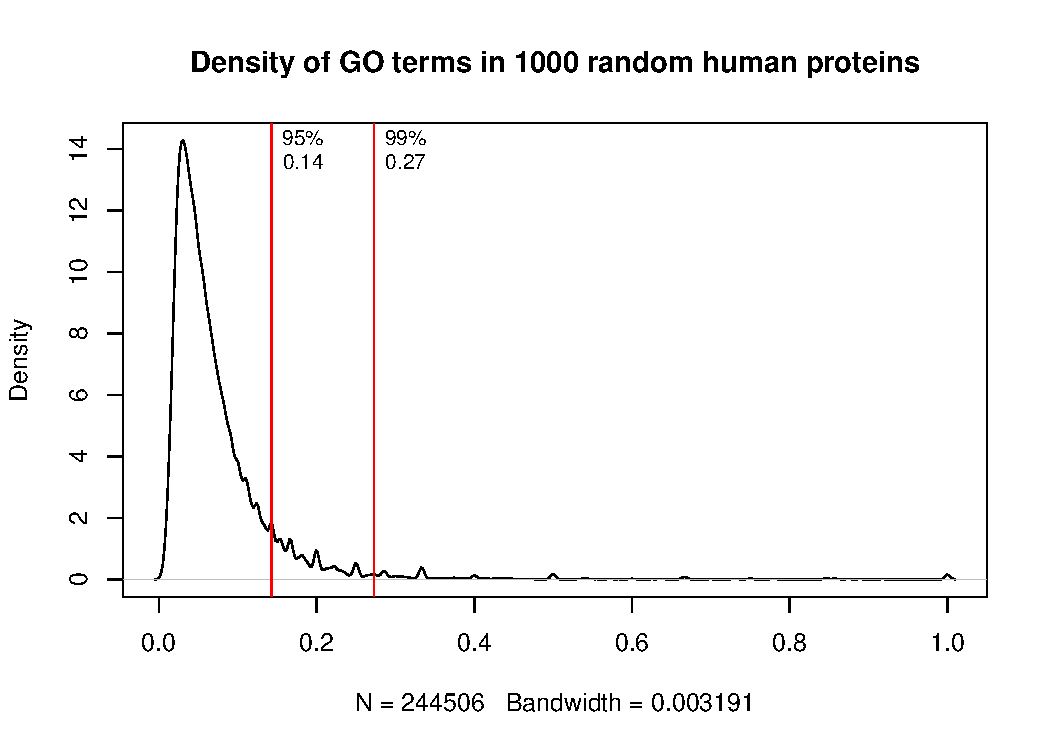
\includegraphics[width=\linewidth]{go_random_density}
\caption{\textbf{The density of GO-terms for 1000 randomly selected proteins.} This density plot shows where the selected cutoffs for GO scores were made. The 95\% quantile and the 99\% quantile were selected. These values were 0.14 and 0.27 respectively.}
\label{fig:go_random_density}
\end{figure}

\subsection{Benchmarking putative homologs}

BLAST and PSI-BLAST E-values were compared to GO homology assignments (\textit{i.e.} different and similar) using Receiver Operator Characteristics (ROC). For a given E-value threshold, protein pairs were classified as following: All positives pairs have an E-value below a threshold, True positives (TP) are similar and false positive (FP) are different according to GO. All negative pairs have an E-value above a threshold. True negatives (TN) are different and false negatives (FN) are similar according to GO. Coverage and error are computed using formulas \eqref{eq:cov} and \eqref{eq:error}.

\begin{subequations}
\begin{align}
Coverage &= \frac{TP}{TP + FN} \label{eq:cov} \\
Error &= \frac{FP}{TN + FP} \label{eq:error}
\end{align}
\end{subequations}

The ROC plot is created by plotting coverage in function of error for different E-value thresholds. A common measure of the accuracy of a method is the Area Under the Curve (AUC) of the ROC plot. The AUC has the advantage of being a point measure bounded between 0 and 1. It was numerically estimated using the trapezoidal method \citep{kaw_numerical_2011}. This method works by taking discrete areas of the function in equal-width trapezoids, then it computes the area of these trapezoids and estimates the AUC as a sum of these discrete areas.

\newpage
\section{Results \& Discussion}

The goal of this study was to benchmark the performance of BLAST and PSI-BLAST in finding homologs using the Gene Ontology database as a gold standard. BLAST and PSI-BLAST E-value distributions are summarized in Figure \ref{fig:blast_evalue_cutoffs}. BLAST and PSI-BLAST results were compared to GO using ROC (Figure \ref{fig:roc_plot_blast}). We report an AUC of 0.676 for BLAST and 0.679 for PSI-BLAST.

\begin{figure}[!hb]
\centering
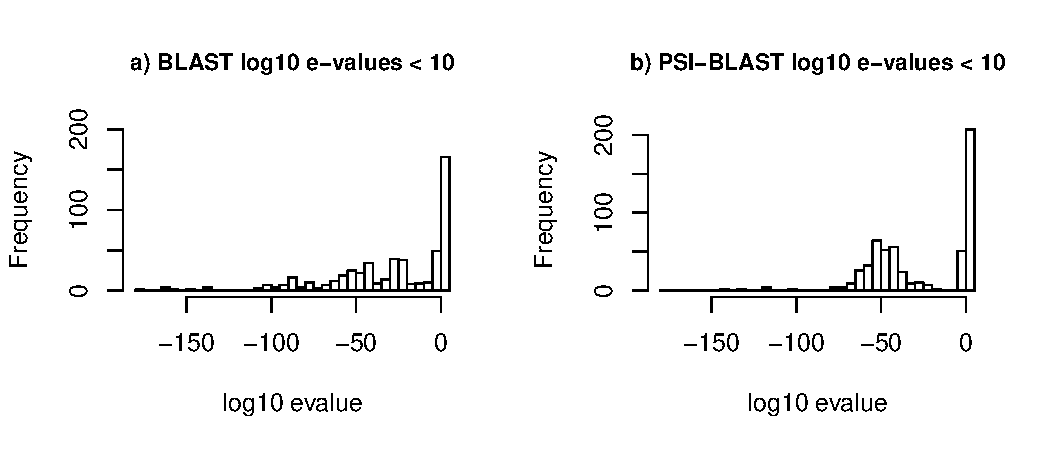
\includegraphics[width=\linewidth]{blast_evalue_cutoffs}
\caption{\textbf{BLAST and PSI-BLAST distributions of decimal logarithmic E-values.} a) Distribution of 543 BLAST E-values spread from $0$ to $10^{-100}$. b) Distribution of 602 PSI-BLAST E-values that are centered around $10^{-50}$.}
\label{fig:blast_evalue_cutoffs}
\end{figure}

\begin{figure}[!ht]

\includegraphics[width=0.9\linewidth]{roc_plot_blast}
\caption{\textbf{Receiver Operator Characteristics (ROC) of BLAST and PSI-BLAST.} This ROC plot illustrates the performance of both BLAST and PSI-BLAST to Gene Ontology as a gold standard. The AUC scores were 0.676 and 0.679 for BLAST and PSI-BLAST respectively, indicating both are above the 0.50 random threshold.}
\label{fig:roc_plot_blast}
\end{figure}

In Figure \ref{fig:roc_plot_blast}, the BLAST and PSI-BLAST results both follow a similar curve. However, at the start of the curve, between 0.15 and 0.4, PSI-BLAST has a higher coverage than BLAST. At a later point in the curve, between 0.6 and 0.8, BLAST has higher coverage than PSI-BLAST. These variations might be attributed to random fluctuations [Q4.2]. These values indicate a higher than random prediction, this is indicated by an AUC of 0.5. In the ROC plot, this is shown by plotting a diagonal line from coordinates (0,0) to (1,1). A perfect method would follow the y-axis vertically from (0,1) and then horizontally follow the x-axis until it reaches (1,1), resulting in an expected AUC of 1 [Q4.1].

The database used to estimate the PSSM influences results. In our study, PSSMs were estimated using a local database of only 209 sequences. It might not contain enough information concerning the amino-acid variation and results in too stringent PSSMs and thus premature convergence of the algorithm. Using a larger database such as the non-redundant UniProt database can influence the obtained E-values. The latter contains more sequences, and will allow a better estimation of the amino acid frequencies in the PSSM. The computed PSSM can then be used to search in the smaller local database and should detect more distant homologs [Q2.8 + Q4.2].

\newpage

Proper estimation of the PSI-BLAST PSSMs also depends on the E-value threshold used for inclusion. High thresholds result in loosely defined PSSMs due to the inclusion of non-homologous proteins. This is also known as profile wander \citep{jaap}. Low thresholds result in stringent PSSMs that do not capture amino-acid variations and premature convergence [Q2.6]. 

PSI-BLAST is usually more sensitive than BLAST because it includes information about amino-acid variation specific to the homologous protein family. BLAST is more specific because it does not consider such variations but only includes the amino-acid substitution matrix \citep{bhagwat_psi-blast_2007}. This explains why PSI-BLAST returns more hits than BLAST. This gain in sensitivity comes at the expense of specificity which is seen in the E-value distributions in figure \ref{fig:blast_evalue_cutoffs} [Q2.7].

We found 87 protein pairs had a PSI-BLAST E-value below $10^{-5}$, but were classified as ``different'' according to GO. For example, the heat shock cognate 71kDa bovine protein (UniprotID: P19120) and heat shock protein homolog SSE1 (Uniprot ID: P32589) had an E-value of zero but a non-significant GO similarity score of 0.125. This leads to the first false positive result in the ROC plot, that can be found at the first horizontal curve around coordinates (0,0.25) in figure \ref{fig:roc_plot_blast} [Q4.3].

Less information is available about biological function than about sequences. There are around 50 million sequences in UniProt \citep{consortium_uniprot:_2015}. The GO database only annotates 400 000 proteins \citep{consortium_gene_2015}. This lack of annotation leads to biased estimations of GO similarity score [Q4.3]. Alternative ways of inferring homology for proteins can be done using protein domains contained in the Pfam database or using structural information using the SCOP database. The pros and cons of these are summarized in table \ref{table:db} [Q4.4]. 

Two genes that share a common ancestor are defined as being true homologs. Depending on which database is used, the assumption of how homology is observed changes. Using GO, the assumption is that homology is linked to functional characteristics. Proteins that share similar functions are likely to have common ancestry. Conversely, a database such as Pfam only looks at sequence domains. The assumption of homology here lies in sequence conservation. Lastly, SCOP looks at protein structure assuming that proteins that have similar structure are likely to have common ancestry [Q4.5]. Every assumption has its merits. Therefore, further studies should define a gold standard based on combining all three databases.

\begin{table}[bh!]
\centering
\caption{\textbf{Pros and cons of the three different databases: GO, Pfam and SCOP.}}
\label{table:db}
\begin{tabular}{|c|p{5cm}|p{5cm}|}
\hline
     & \textbf{Pros}                                                                            & \textbf{Cons}                                                                            \\ \hline
\textbf{GO}   &  -Looks at biological function which is more conserved than  &  -Only 400,000 annotated proteins                                                 \\ 
     & sequence                                                                                &  -Susceptible to classify convergent evolution as homology \\ \hline
\textbf{Pfam} &  -Large database covering ~80\% of UniProt (~40 million proteins)                 &  -Only looks at sequence that is less conserved                                \\ \hline
\textbf{SCOP} &  -Looks at structure which is more conserved than sequence                        &  -Structure data is sparse, limited data available (~40,000 proteins)
\\ 
     &                                                                                 &  -More susceptible to classify similarity due to convergent evolution as homology \\ \hline
\end{tabular}
\end{table}

\newpage
\section{Conclusion}

The aim of our study was to benchmark BLAST and PSI-BLAST as a homology search tool using GO as a gold standard. Our results indicate that BLAST and PSI-BLAST have low and similar accuracy for homology prediction. Therefore we can conclude that BLAST and PSI-BLAST perform far from optimal in searching for homologs. However taking into account the 87 pairs of false positives with low BLAST and PSI-BLAST E-values, GO is probably not yet annotated enough to serve as a homology benchmarking standard.

\newpage
\bibliographystyle{plainnat}
\bibliography{biblio}

\end{document}
